\section{Heterogeneous Networks and the Gateway Bridge}
Consider the typical hourglass network stack in IP-based networks as shown in left-hand image of Figure \ref{fig:hourglass}. This layered design with a thin-waist infrastructure (IP packets for traffic flow) is what enabled the Internet to grow and expand at such a rapid rate; higher layers in the protocol stack extend this communication medium with support for a variety of applications and networking features (e.g., reliable message traversal via TCP). While the NDN architecture introduces a fundamental paradigm shift in the way information is published and retrieved on a network, its design, shown at a high level in the right-hand image of Figure \ref{fig:hourglass}, borrows the same hourglass design as IP networks. Observe that upper layers of the network stack still promote the development of robust applications based on the underlying communication layers. The difference, however, is that network traffic flow management (i.e., to enable reliable and stable communication) and security are \emph{built into} the network stack. These architectural differences mean that application, transport, and network layer protocol semantics in IP-based networks are distinct from protocol semantics in NDN networks. The NDN gateway is intended to bridge between IP and NDN networks by performing this semantic translation between protocols. 

\begin{figure}
\begin{center}
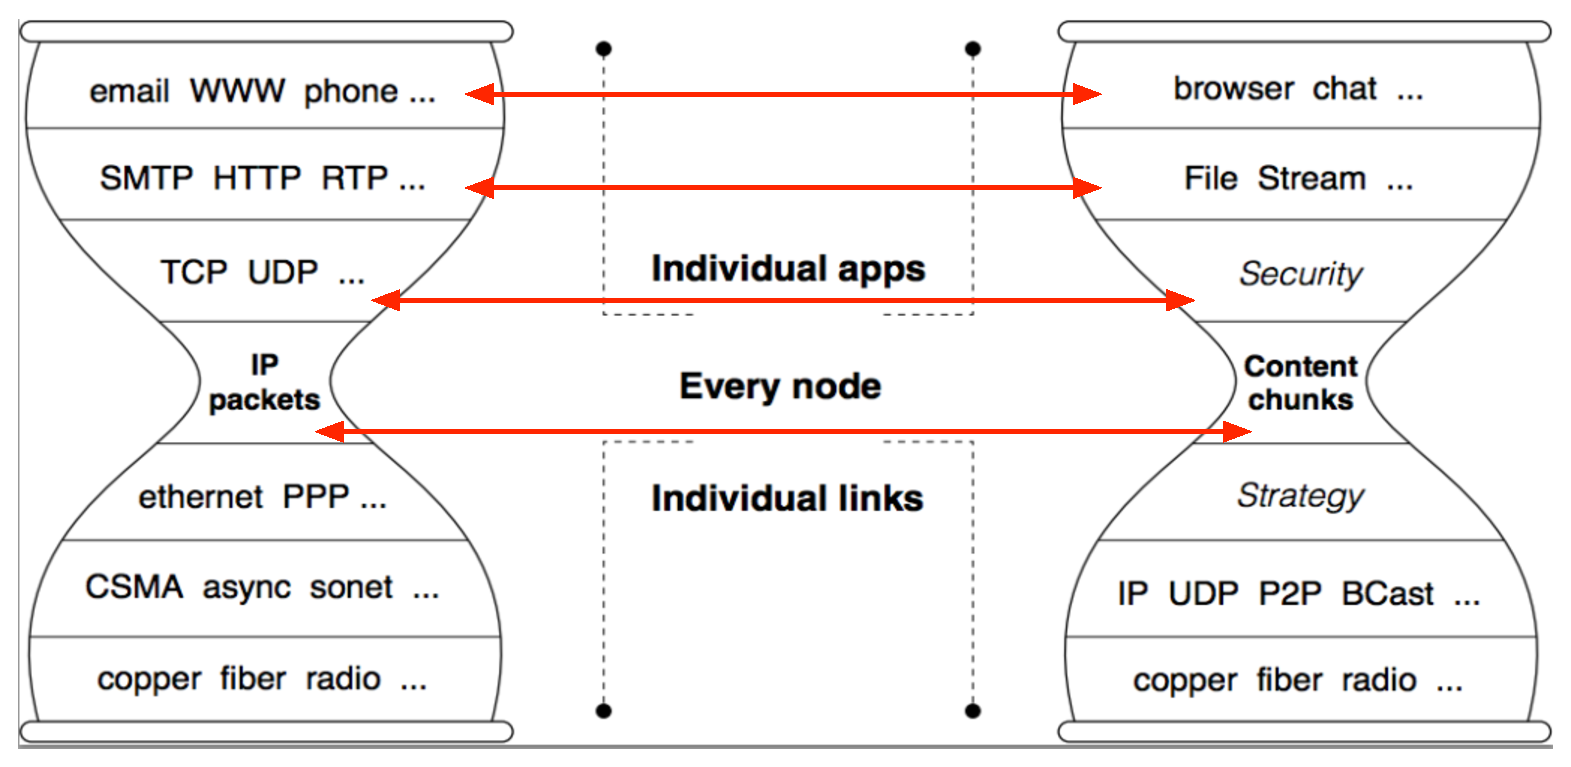
\includegraphics[scale=0.5]{./images/hourglass_conn.pdf}
\label{fig:hourglass}
\caption{TODO}
\end{center}
\end{figure}

The gateway middleware is designed so as to support bi-directional traffic flowing from both types of networks. In what follows we describe how traffic in both directions will be supported internally by the gateway.

\begin{table}[t]
    \begin{tabular}{|c||c|c|}
    \hline
    ~    & {\bf IP} & {\bf NDN} \\ \hline
    {\bf HTTP} & ~ & ~ \\ \hline
    {\bf FTP}  & ~ & ~ \\ \hline
    {\bf SMTP} & ~ & ~ \\ \hline
    {\bf DNS}  & ~ & ~ \\ \hline
    \end{tabular}
\end{table}

\subsection{IP-to-NDN Traffic}
TODO

\subsection{NDN-to-IP Traffic}
TODO